% This file was created by tikzplotlib v0.9.4.
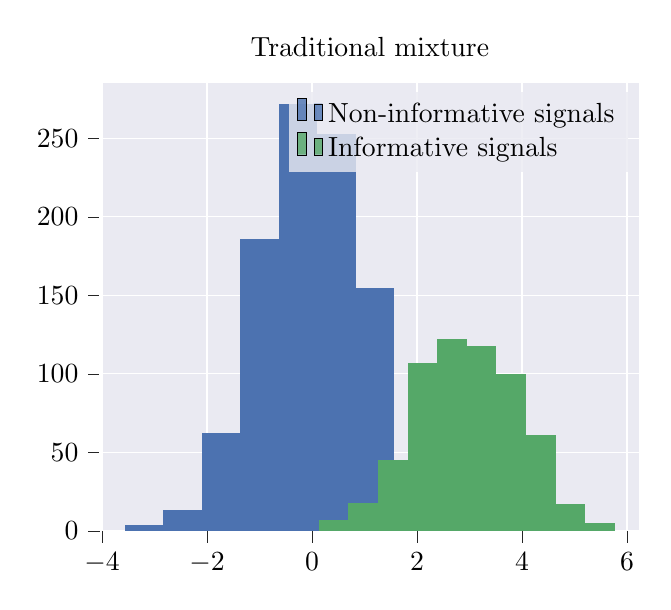
\begin{tikzpicture}

\definecolor{color0}{rgb}{0.917647058823529,0.917647058823529,0.949019607843137}
\definecolor{color1}{rgb}{0.298039215686275,0.447058823529412,0.690196078431373}
\definecolor{color2}{rgb}{0.333333333333333,0.658823529411765,0.407843137254902}

\begin{axis}[
axis background/.style={fill=color0},
axis line style={white},
legend cell align={left},
legend style={fill opacity=0.8, draw opacity=1, text opacity=1, draw=none, fill=color0},
tick align=outside,
tick pos=left,
title={Traditional mixture},
x grid style={white},
xmajorgrids,
xmin=-4.03741023632269, xmax=6.24055737734554,
xtick style={color=white!15!black},
y grid style={white},
ymajorgrids,
ymin=0, ymax=285.6,
ytick style={color=white!15!black}
]
\draw[draw=none,fill=color1,line width=0.12pt] (axis cs:-3.57022989024686,0) rectangle (axis cs:-2.83701113466794,4);
\addlegendimage{ybar,ybar legend,draw=none,fill=color1,line width=0.12pt};
\addlegendentry{Non-informative signals}

\draw[draw=none,fill=color1,line width=0.12pt] (axis cs:-2.83701113466794,0) rectangle (axis cs:-2.10379237908901,13);
\draw[draw=none,fill=color1,line width=0.12pt] (axis cs:-2.10379237908901,0) rectangle (axis cs:-1.37057362351009,62);
\draw[draw=none,fill=color1,line width=0.12pt] (axis cs:-1.37057362351009,0) rectangle (axis cs:-0.637354867931162,186);
\draw[draw=none,fill=color1,line width=0.12pt] (axis cs:-0.637354867931162,0) rectangle (axis cs:0.0958638876477624,272);
\draw[draw=none,fill=color1,line width=0.12pt] (axis cs:0.0958638876477624,0) rectangle (axis cs:0.829082643226687,253);
\draw[draw=none,fill=color1,line width=0.12pt] (axis cs:0.829082643226687,0) rectangle (axis cs:1.56230139880561,155);
\draw[draw=none,fill=color1,line width=0.12pt] (axis cs:1.56230139880561,0) rectangle (axis cs:2.29552015438454,44);
\draw[draw=none,fill=color1,line width=0.12pt] (axis cs:2.29552015438454,0) rectangle (axis cs:3.02873890996346,10);
\draw[draw=none,fill=color1,line width=0.12pt] (axis cs:3.02873890996346,0) rectangle (axis cs:3.76195766554239,1);
\draw[draw=none,fill=color2,line width=0.12pt] (axis cs:0.124909566278549,0) rectangle (axis cs:0.689756312777664,7);
\addlegendimage{ybar,ybar legend,draw=none,fill=color2,line width=0.12pt};
\addlegendentry{Informative signals}

\draw[draw=none,fill=color2,line width=0.12pt] (axis cs:0.689756312777664,0) rectangle (axis cs:1.25460305927678,18);
\draw[draw=none,fill=color2,line width=0.12pt] (axis cs:1.25460305927678,0) rectangle (axis cs:1.8194498057759,45);
\draw[draw=none,fill=color2,line width=0.12pt] (axis cs:1.8194498057759,0) rectangle (axis cs:2.38429655227501,107);
\draw[draw=none,fill=color2,line width=0.12pt] (axis cs:2.38429655227501,0) rectangle (axis cs:2.94914329877413,122);
\draw[draw=none,fill=color2,line width=0.12pt] (axis cs:2.94914329877413,0) rectangle (axis cs:3.51399004527324,118);
\draw[draw=none,fill=color2,line width=0.12pt] (axis cs:3.51399004527324,0) rectangle (axis cs:4.07883679177236,100);
\draw[draw=none,fill=color2,line width=0.12pt] (axis cs:4.07883679177236,0) rectangle (axis cs:4.64368353827147,61);
\draw[draw=none,fill=color2,line width=0.12pt] (axis cs:4.64368353827147,0) rectangle (axis cs:5.20853028477059,17);
\draw[draw=none,fill=color2,line width=0.12pt] (axis cs:5.20853028477059,0) rectangle (axis cs:5.77337703126971,5);
\end{axis}

\end{tikzpicture}
